\documentclass[11pt]{article}
%Gummi|065|=)

\usepackage{array}
\usepackage{graphicx}
\usepackage{tgschola}
\usepackage{algorithmic}
\usepackage{amssymb}
\usepackage{amsmath}
\DeclareMathOperator*{\argmax}{argmax}

\title{\textbf{SSU : Assignment 3} \\ \textbf{Digit recognition using Convolutional neural networks}}
\author{\textbf{Teymur Azayev}}
\date{}


\begin{document}

\maketitle

\section{Overview}
This document is a short report for the third assignment from the subject. It includes a theoretical overview of the task, an explanation of the implementation, results and a short discussion.

\section{Task}
The task is to train a small convolutional neural network on a commonly used dataset named MNIST.
This dataset consists of images of digits 0 to 9 inclusive.
We will first train the network on a subset of the dataset, namely digits 6 to 9 with various proportions,
noting the generalization accuracy after having trained on each proportion.
We will then train the network on the complete subset of digits 0 to 5 and then reuse the convolutional
layers for the training of digits 6 to 9, demonstrating the efficiency of transfer learning.

\section{Implementation and results} 
The convolutional neural network is implemented in python using tensorflow. The architecture is specified in the 
given task so it will not be mentioned here. We use a batchsize of 100 and an ADAM optimizer with an $\alpha$ of $0.001$, except in the finetuning where a rate of $\alpha = 0.0003$ is used. The network weights are initialized randomly using the standard Xavier initialization. Each configuration was trained 10 times for a total of 1000 iterations and an average of the test accuracies is obtained. The following figure shows the result trained on the 6 to 9 digits with various proportions.


% Include image on raw 69 here
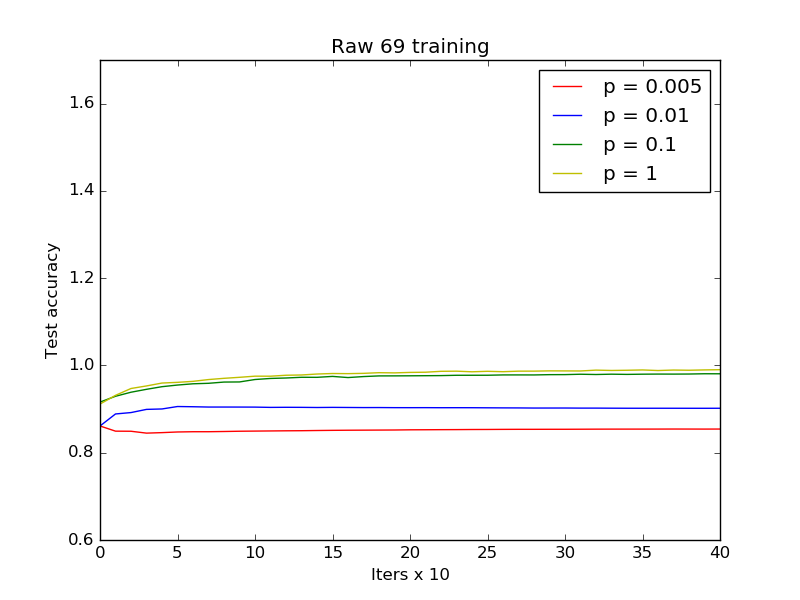
\includegraphics[width=10cm]{Raw69training}

We can how the accuracies are high after even before the first test evaluation. This is because MNIST is a very easy dataset and we can start classifying successfully even after a couple of hundred examples. We can note how test accuracy for the lower proportion drops because we are overfitting the data after some time.\\

The network is now trained on the 0 to 5 digits. We now freeze the convolutional layers (not allow gradients to flow through them) and retrain the network on digits 6 to 9. The following figure demonstrates the results \\ 

% Insert the retrained network results on the 6 to 9
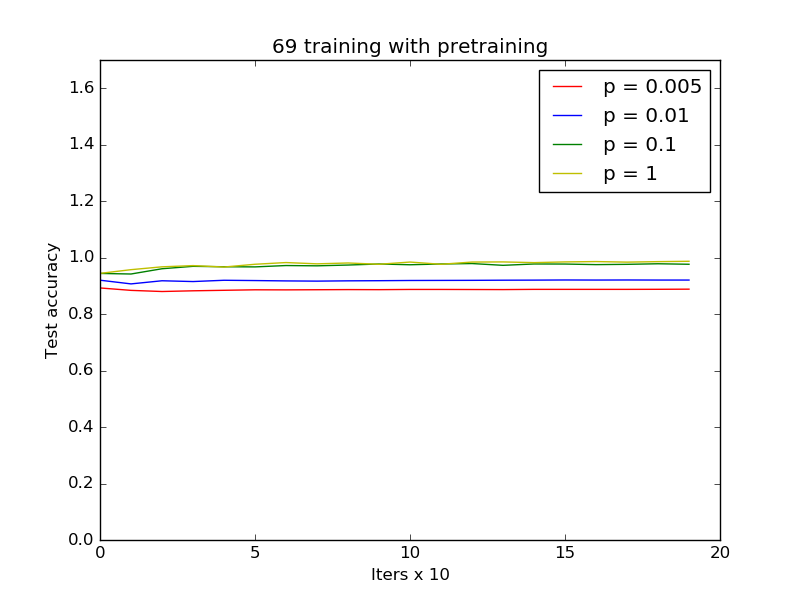
\includegraphics[width=10cm]{69trainingwithpretraining}

We can see that the network has a high accuracy very early and does not improve that much over time.
Also, it should be noted that the proportions with a lower amount of samples are now doing slightly better. This is one of the key features of transfer learning. We can also try to retrain the network using pretrained features, but this time without freezing the convolutional layers. A slightly lower learning rate is used for this session.

% Insert the retrained network finetuned results on the 6 to 9
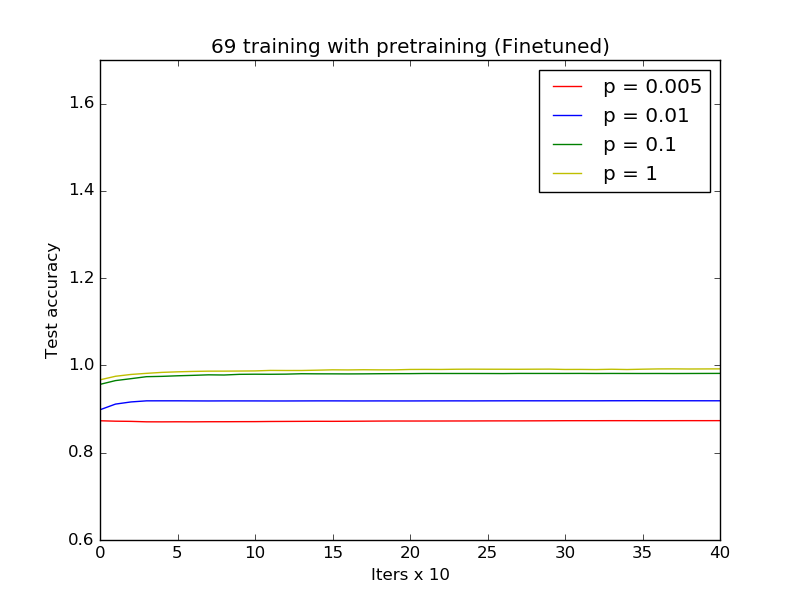
\includegraphics[width=10cm]{69trainingwithpretraining(Finetuned)}

\section{Use of regularization}
Using the finetuning we can get an overall higher test accuracy.
We will now add the dropout technique to the fully connected layers of the network as a method of regularization.
A keep probability of 0.5 is used. We can see that we need less iterations than without dropout for the network to get good results. Dropout also helps with overfitting and finds more robust features by eliminating neuron co-firing, esentially introducing random noise.

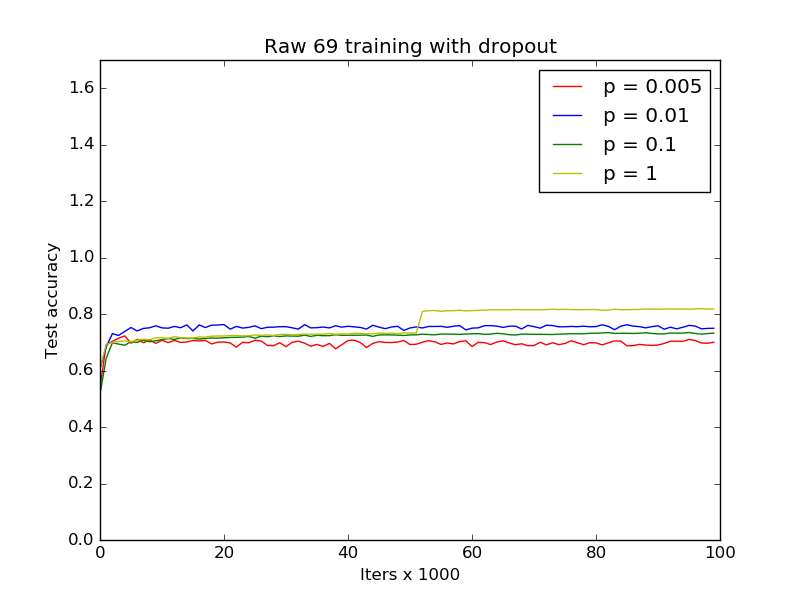
\includegraphics[width=10cm]{Raw69trainingwithdropout}

\section{Test accuracies}
The following table summarizes the test accuracies on the whole 6-9 dataset
for each of the models for all proportions \\ 

\begin{tabular}{ |p{4cm}||p{2cm}|p{2cm}|p{2cm}|p{2cm}| }
 \hline
 \multicolumn{5}{|c|}{Test accuracies} \\
 \hline
Model & p = 0.005 & p = 0.01 & p = 0.1 & p = 1\\
 \hline
 Raw 69                       &   0.8559     & 0.9016    &  0.9806   & 0.9919\\
 69 /w pretr.                 &   0.8846     & 0.9203    &  0.9814   & 0.9926\\
 69 /w pretr. /w Finetune     &   0.8750     & 0.9194    &  0.9821   & 0.9932\\
 69 Dropout                   &   0.8778     & 0.9194    &  0.9845   & 0.9927\\
 \hline
\end{tabular}

\section{Discussion}
We saw that using a higher proportion of data leads to smaller test error (better generalization). 
We also demonstrated the effectiveness of transfer learning where we used a network which was trained on 
one dataset as a feature extractor on top of which we trained another network. We can see that this 
method alleviates the need for large datasets which is a typical problem with deep learning. 
From the table it can also be noted that using dropout gives us better results than without regularization.
The highest test accuracy was measured using pretraining and fine tuning.


\section{Conclusion}
This concludes the report on this task.


\end{document}
